\documentclass[aspectratio=169]{beamer}
\usepackage[utf8]{inputenc}
\usepackage{lmodern}
\usepackage{tikz}
\usepackage{hyperref}
\usetikzlibrary{positioning,shapes.geometric,arrows.meta}

\definecolor{skyblue}{HTML}{56C6F4}
\definecolor{sunnyyellow}{HTML}{FFD84D}
\definecolor{coral}{HTML}{FF7F6E}
\definecolor{leafgreen}{HTML}{67C587}
\definecolor{ink}{HTML}{213547}
\definecolor{cloud}{HTML}{F7FBFF}
\definecolor{lavender}{HTML}{E9E1FF}

\setbeamertemplate{navigation symbols}{}
\setbeamercolor{normal text}{fg=ink,bg=white}
\setbeamercolor{frametitle}{fg=ink,bg=white}
\setbeamercolor{title}{fg=ink}
\setbeamercolor{block title}{fg=white,bg=coral}
\setbeamercolor{block body}{fg=ink,bg=cloud}
\setbeamercolor{alertblock title}{fg=white,bg=leafgreen!75!black}
\setbeamercolor{alertblock body}{fg=ink,bg=leafgreen!10}
\setbeamercolor{palette primary}{fg=white,bg=coral}
\setbeamertemplate{itemize item}{\color{coral}$\blacktriangleright$}
\setbeamertemplate{enumerate item}{\color{coral}\insertenumlabel.}
\setbeamerfont{title}{series=\bfseries,size=\Huge}
\setbeamerfont{frametitle}{series=\bfseries,size=\Large}
\setbeameroption{hide notes}

\newcommand{\stepbadge}[3]{%
  \begin{tikzpicture}[baseline=(box.center)]
    \node[rounded corners=10pt, fill=#1, minimum width=2.4cm, minimum height=0.85cm] (box)
    {\color{white}\bfseries #2};
    \node[right=0.18cm of box, anchor=west] {\color{ink}\bfseries #3};
  \end{tikzpicture}
}

\title{Boxitects \& Beyond}
\subtitle{Bright, Step-by-Step Student Guide}
\author{Pine Brook IGNITE}
\date{Spring 2026}

\begin{document}

\begin{frame}[plain]

\begin{tikzpicture}[remember picture,overlay]
  \fill[cloud] (current page.south west) rectangle (current page.north east);
  \fill[sunnyyellow!50] (-0.2,7.4) rectangle (13.6,7.8);
  \fill[skyblue!22] (-0.2,-0.2) rectangle (13.6,1.3);
  \fill[coral!18] (0.4,5.4) circle (0.65);
  \fill[leafgreen!18] (12.4,6.2) circle (0.5);
  \fill[lavender!55] (11.6,1.0) circle (0.45);
  \fill[sunnyyellow!70] (1.2,1.0) circle (0.35);
\end{tikzpicture}

\vspace{0.35cm}
\begin{center}
{\Huge\bfseries\color{ink} Boxitects \& Beyond\par}
\vspace{0.2cm}
{\Large\color{coral} Plan it. Make it. Share it.\par}
\vspace{0.35cm}


\begin{tikzpicture}
\node[rounded corners=18pt, fill=skyblue!18, draw=skyblue!60, line width=1.2pt,
      minimum width=11.2cm, minimum height=1.5cm, text width=10.2cm, align=center]
      {\Large\bfseries Bright cues, repeated colors, and short steps help this class keep going with confidence.};
\end{tikzpicture}

\vspace{0.35cm}

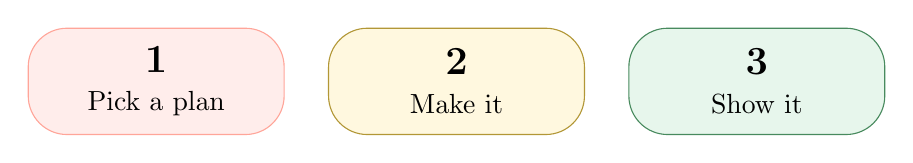
\begin{tikzpicture}[node distance=0.55cm]
\node[draw=coral!70, fill=coral!14, rounded corners=14pt, minimum width=3.25cm, minimum height=1.35cm, align=center] (a) {\Large\bfseries 1\\[2pt]Pick a plan};
\node[draw=sunnyyellow!70!black, fill=sunnyyellow!18, rounded corners=14pt, minimum width=3.25cm, minimum height=1.35cm, align=center, right=of a] (b) {\Large\bfseries 2\\[2pt]Make it};
\node[draw=leafgreen!70!black, fill=leafgreen!16, rounded corners=14pt, minimum width=3.25cm, minimum height=1.35cm, align=center, right=of b] (c) {\Large\bfseries 3\\[2pt]Show it};
\end{tikzpicture}
\end{center}
\note{Today we are working on boxitects \& beyond}
\end{frame}

\begin{frame}[plain]
\frametitle{What Are We Doing Today?}
\begin{columns}[T,totalwidth=\textwidth]
\column{0.56\textwidth}
\begin{block}{Our Goal}
\Large Boxitects Video or Book
\end{block}
\vspace{0.15cm}
{\large\bfseries\color{coral} Success looks like this:}
\begin{itemize}\large
\item Boxitects Video or Book
\item Chart Paper \& markers
\item Variety of building materials
\end{itemize}
\column{0.4\textwidth}
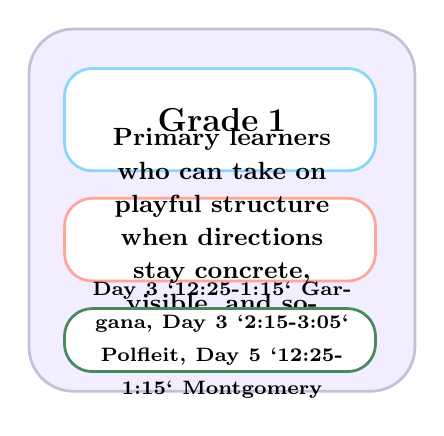
\begin{tikzpicture}[x=1cm,y=1cm]
\draw[rounded corners=16pt, fill=lavender!55, draw=lavender!85!black, line width=1pt] (0,0) rectangle (4.9,4.6);
\draw[rounded corners=10pt, fill=white, draw=skyblue!70, line width=1pt] (0.45,2.8) rectangle (4.4,4.1);
\node[align=center, text width=3.3cm] at (2.45,3.45) {\large\bfseries Grade 1};
\draw[rounded corners=10pt, fill=white, draw=coral!70, line width=1pt] (0.45,1.4) rectangle (4.4,2.45);
\node[align=center, text width=3.3cm] at (2.45,1.93) {\small\bfseries Primary learners who can take on playful structure when directions stay concrete, visible, and socially supported.};
\draw[rounded corners=10pt, fill=white, draw=leafgreen!70!black, line width=1pt] (0.45,0.25) rectangle (4.4,1.05);
\node[align=center, text width=3.3cm] at (2.45,0.65) {\scriptsize\bfseries Day 3 `12:25-1:15` Gargana, Day 3 `2:15-3:05` Polfleit, Day 5 `12:25-1:15` Montgomery};
\end{tikzpicture}
\end{columns}
\note{Today we are working on boxitects \& beyond}
\end{frame}

\begin{frame}[plain]
\frametitle{What You Need}
\begin{columns}[T,totalwidth=\textwidth]
\column{0.6\textwidth}
\stepbadge{skyblue}{READY}{Get set}
\vspace{0.18cm}
\begin{itemize}\large
\item Begin by naming the lesson purpose and the success condition
\item Model the first step before independent or partner work starts
\item Pause once mid-lesson for a quick debug, reflection, or reset
\end{itemize}
\vspace{0.2cm}
\stepbadge{leafgreen}{TEAM}{How we work}
\vspace{0.18cm}
\begin{itemize}\large
\item Look
\item Listen
\item Try
\item Help without taking over
\end{itemize}
\column{0.35\textwidth}
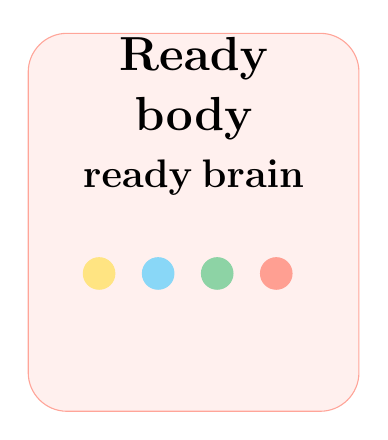
\begin{tikzpicture}[x=1cm,y=1cm]
\node[draw=coral!70, fill=coral!12, rounded corners=14pt, minimum width=4.2cm, minimum height=4.8cm] {};
\node[align=center, text width=3.4cm] at (0,1.35) {\LARGE\bfseries Ready body\\[6pt]\Large ready brain};
\draw[fill=sunnyyellow!70, draw=sunnyyellow!70] (-1.2,-0.65) circle (0.2);
\draw[fill=skyblue!70, draw=skyblue!70] (-0.45,-0.65) circle (0.2);
\draw[fill=leafgreen!75, draw=leafgreen!75] (0.3,-0.65) circle (0.2);
\draw[fill=coral!75, draw=coral!75] (1.05,-0.65) circle (0.2);
\end{tikzpicture}
\end{columns}
\note{Set materials before noise grows. Keep the routine visible.}
\end{frame}

\begin{frame}[plain]
\frametitle{Our Big Plan}
\begin{center}
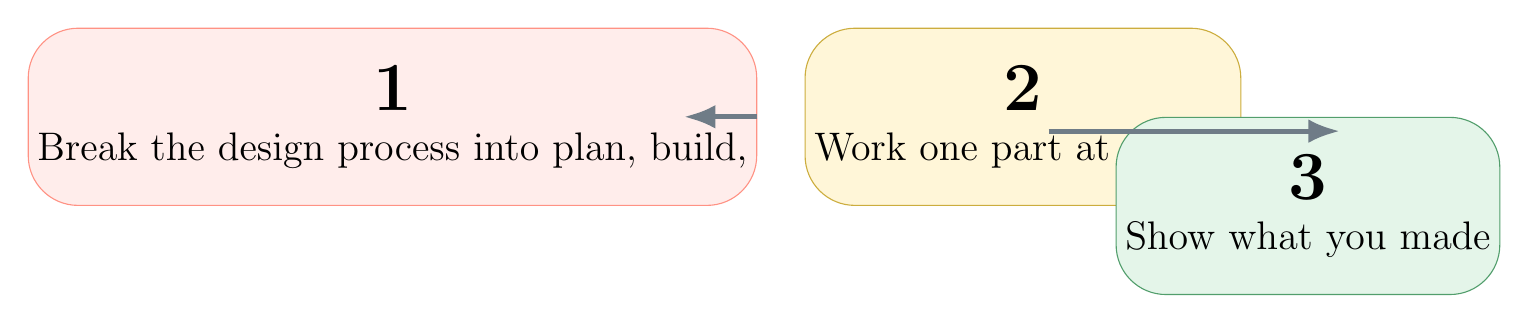
\begin{tikzpicture}[node distance=0.6cm]
\node[rounded corners=18pt, draw=coral!85, fill=coral!14, minimum width=3.35cm, minimum height=2.25cm, align=center] (s1)
{\Huge\bfseries 1\\[6pt]\Large Break the design process into plan, build,};
\node[rounded corners=18pt, draw=sunnyyellow!80!black, fill=sunnyyellow!22, minimum width=3.35cm, minimum height=2.25cm, align=center, right=of s1]
{\Huge\bfseries 2\\[6pt]\Large Work one part at a time};
\node[rounded corners=18pt, draw=leafgreen!80!black, fill=leafgreen!18, minimum width=3.35cm, minimum height=2.25cm, align=center, right=of s1.south east, xshift=3.95cm, yshift=0.0cm]
{\Huge\bfseries 3\\[6pt]\Large Show what you made};
\draw[-{Latex[length=4mm,width=3mm]}, line width=1.8pt, color=ink!65] (s1) -- ++(3.7,0);
\draw[-{Latex[length=4mm,width=3mm]}, line width=1.8pt, color=ink!65] (s1.south east) ++(3.7,0.95) -- ++(3.7,0);
\end{tikzpicture}
\end{center}
\vspace{0.28cm}
\begin{block}{Keep your eyes on the color}
\Large Red means begin. Yellow means work. Green means show.
\end{block}
\note{Use the help routine before you panic}
\end{frame}

\begin{frame}[plain]
\frametitle{If You Get Stuck}
\begin{columns}[T,totalwidth=\textwidth]
\column{0.54\textwidth}
\begin{alertblock}{Our Help Ladder}
\Large Try the next small support before you freeze.
\end{alertblock}
\begin{enumerate}\large
\item Look at the slide.
\item Look at your checklist.
\item Ask your partner.
\item Ask the teacher one clear question.
\end{enumerate}
\vspace{0.18cm}
{\large\bfseries\color{coral} Watch for this:}
\begin{itemize}\large
\item Some groups need support organizing materials and sticking with one plan
\item Explaining the design can be harder than making it without sentence
\item Students may not know they are done
\end{itemize}
\column{0.4\textwidth}
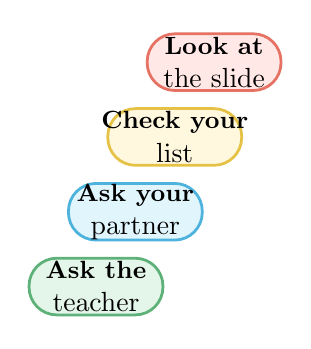
\begin{tikzpicture}[x=1cm,y=1cm]
\draw[rounded corners=10pt, fill=leafgreen!18, draw=leafgreen!90!black, line width=1pt] (0.2,0.2) rectangle (1.9,0.92);
\node[align=center] at (1.05,0.56) {\small\bfseries Ask the\\teacher};
\draw[rounded corners=10pt, fill=skyblue!18, draw=skyblue!90!black, line width=1pt] (0.7,1.15) rectangle (2.4,1.87);
\node[align=center] at (1.55,1.51) {\small\bfseries Ask your\\partner};
\draw[rounded corners=10pt, fill=sunnyyellow!18, draw=sunnyyellow!90!black, line width=1pt] (1.2,2.1) rectangle (2.9,2.82);
\node[align=center] at (2.05,2.46) {\small\bfseries Check your\\list};
\draw[rounded corners=10pt, fill=coral!18, draw=coral!90!black, line width=1pt] (1.7,3.05) rectangle (3.4,3.77);
\node[align=center] at (2.55,3.41) {\small\bfseries Look at\\the slide};
\end{tikzpicture}
\end{columns}
\note{Use the help routine before you panic}
\end{frame}

\begin{frame}[plain]
\frametitle{Before We Finish}
\begin{center}
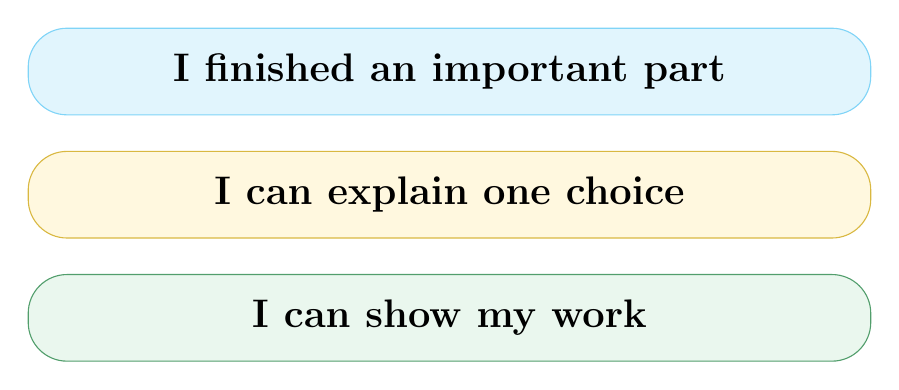
\begin{tikzpicture}[node distance=0.45cm]
\node[rounded corners=14pt, fill=skyblue!18, draw=skyblue!75, minimum width=10.7cm, minimum height=1.1cm, align=center] (a) {\Large\bfseries I finished an important part};
\node[rounded corners=14pt, fill=sunnyyellow!18, draw=sunnyyellow!85!black, minimum width=10.7cm, minimum height=1.1cm, align=center, below=of a] (b) {\Large\bfseries I can explain one choice};
\node[rounded corners=14pt, fill=leafgreen!14, draw=leafgreen!80!black, minimum width=10.7cm, minimum height=1.1cm, align=center, below=of b] (c) {\Large\bfseries I can show my work};
\end{tikzpicture}
\end{center}
\vspace{0.3cm}
\begin{block}{Exit move}
\Large Save it, hold it up, point to it, or explain it.
\end{block}
\note{Show what you learned at the end}
\end{frame}

\end{document}
